\documentclass[12pt,oneside]{report}
\usepackage[utf8]{inputenc}
\usepackage[brazil]{babel}
\usepackage[T1]{fontenc}
\usepackage{graphicx}
\usepackage{amsmath}
\usepackage{longtable}
\usepackage{float}
\usepackage{indentfirst}
\usepackage{array}
\usepackage{fancyhdr}
\usepackage{amsmath,amssymb}
\usepackage{csquotes}
\usepackage{tocloft}
\usepackage[nottoc]{tocbibind}
\usepackage[a4paper,top=3cm,bottom=2cm,left=3cm,right=2cm]{geometry}
\usepackage{titlesec}
\usepackage{caption}
\usepackage{setspace}
\usepackage{lmodern}
\usepackage{changepage}
\usepackage{tabularx}
\usepackage[backend=biber,style=abnt]{biblatex}

\usepackage[colorlinks=true, linkcolor=black, citecolor=black, urlcolor=blue]{hyperref}
\usepackage{booktabs}

\setlength{\parindent}{2em}
\setlength{\parskip}{0.5em}

\renewcommand{\cftchapleader}{\cftdotfill{\cftdotsep}}
\renewcommand{\listfigurename}{Lista de Ilustrações}
\renewcommand{\arraystretch}{1.5}

\addbibresource{referencias.bib}

\titleformat{\chapter}[hang]{\normalfont\bfseries\Large}{\thechapter}{0.5em}{}
\titleformat{\section}{\normalfont\bfseries}{\thesection}{1em}{}
\titleformat{\subsection}{\normalfont\bfseries}{\thesubsection}{1em}{}
\titleformat{\subsubsection}{\normalfont\bfseries}{\thechapter}{1em}{}

\captionsetup[figure]{labelfont=bf,labelsep=endash,name=Figura}
\captionsetup[table]{labelfont=bf,labelsep=endash,name=Tabela}

\begin{document}
\onehalfspacing

% Capa
\begin{titlepage}
    \begin{center}
        \large
        UNIVERSIDADE FEDERAL DO RIO DE JANEIRO \\
        ESCOLA DE QUÍMICA

        \vspace{2cm}

        \textbf{Alex Matos da Silva}

        \vspace{2cm}

        \begin{figure}[htp]
            \centering
            
\includegraphics[width=4cm]{Logo-EQ.jpg}
        \end{figure}

        \vspace{2cm}

        \textbf{\Large DESENVOLVIMENTO DE SOFTWARE PARA SIMULAÇÃO DE PROCESSOS ENZIMÁTICOS}

        \vfill

        RIO DE JANEIRO \\
        2025
    \end{center}
\end{titlepage}

% Folha de rosto
\begin{titlepage}
    \begin{center}
        \textbf{Alex Matos da Silva}

        \vfill

        \textbf{\Large DESENVOLVIMENTO DE SOFTWARE PARA SIMULAÇÃO DE PROCESSOS ENZIMÁTICOS}

        \vfill

        Trabalho de Conclusão de Curso apresentado à Escola de Química da Universidade Federal do Rio de Janeiro, como parte dos requisitos necessários à obtenção do grau de Engenheiro Químico.

        \vfill

        Orientadores: Heloísa Lajas Sanches Fernandes, Bernardo Dias Ribeiro

        \vfill

        Rio de Janeiro \\
        2025
    \end{center}
\end{titlepage}

% Ficha catalográfica (substituir manualmente após gerar)
\newpage
\pagenumbering{roman}
\vspace*{\fill}
\begin{center}
    \textit{Gerar a ficha catalográfica em http://fichacatalografica.sibi.ufrj.br/ e inserir aqui.}
\end{center}
\vspace*{\fill}
\newpage

% Folha de aprovação
\begin{center}
    \textbf{Alex Matos da Silva}

    \vspace{1cm}

    \textbf{DESENVOLVIMENTO DE SOFTWARE PARA SIMULAÇÃO DE PROCESSOS ENZIMÁTICOS}

    \vspace{0.5cm}

    \begin{adjustwidth}{8cm}{0cm}
        Trabalho de Conclusão de Curso apresentado à Escola de Química da Universidade Federal do Rio de Janeiro, como parte dos requisitos necessários à obtenção do grau de Engenheiro Químico.
    \end{adjustwidth}

    \vspace{0.5cm}

\end{center}

Aprovado em 20 de agosto de 2025.

\begin{center}

    \vspace{2cm}

    \noindent\rule{10cm}{0.4pt}\\
    \noindent\hspace*{0.2cm}Heloísa Lajas Sanches Fernandes, D.Sc

    \vspace{1cm}

    \noindent\rule{10cm}{0.4pt}\\
    \noindent\hspace*{0.2cm}Bernardo Dias Ribeiro, D.Sc

    \vspace{2cm}

    \noindent\rule{10cm}{0.4pt}\\
    \noindent\hspace*{0.2cm}Nome (COMPLETO) do Avaliador 1, titulação, instituição

    \vspace{1cm}

    \noindent\rule{10cm}{0.4pt}\\
    \noindent\hspace*{0.2cm}Nome (COMPLETO) do Avaliador 2, titulação, instituição


    \vfill

    Rio de Janeiro \\
    2025
\end{center}
\newpage

% Dedicatória (opcional)
\chapter*{Dedicatória}
\vspace*{\fill}
\begin{center}
    Texto da dedicatória.
\end{center}
\vspace*{\fill}

% Agradecimentos (opcional)
\chapter*{Agradecimentos}
Inserir aqui os agradecimentos.

% Epígrafe (opcional)
\chapter*{Epígrafe}
\vspace*{\fill}
\begin{flushright}
    Texto da epígrafe.
\end{flushright}
\vspace*{\fill}

% Resumo
\chapter*{\MakeUppercase{Resumo}}
SILVA, Alex Matos da. \textbf{Desenvolvimento de Software para Simulação de Processos Enzimáticos}. Rio de Janeiro, 2025. Trabalho de Conclusão de Curso (Graduação em Engenharia Química) – Escola de Química, Universidade Federal do Rio de Janeiro, 2025.

\medskip

[Inserir texto do resumo em português aqui.]

\medskip

\textbf{Palavras-chave}: palavra-chave 1; palavra-chave 2; palavra-chave 3.

% Abstract
\chapter*{\MakeUppercase{Abstract}}
SILVA, Alex Matos da. \textbf{Desenvolvimento de Software para Simulação de Processos Enzimáticos}. Rio de Janeiro, 2025. Trabalho de Conclusão de Curso (Graduação em Engenharia Química) – Escola de Química, Universidade Federal do Rio de Janeiro, 2025.

\medskip

[Insert English abstract here.]

\medskip

\textbf{Keywords}: keyword 1; keyword 2; keyword 3.
\newpage

% Listas
\listoffigures
\newpage

\listoftables
\newpage

% Lista de siglas
\chapter*{Lista de Abreviaturas e Siglas}
\addcontentsline{toc}{chapter}{Lista de Abreviaturas e Siglas}
\begin{tabbing}
    AC \hspace{2cm} \= Autômato Celular \\
    CA \> Cellular Automaton \\
    CSTR \> Continuous Stirred-Tank Reactor \\
    EDO \> Equação Diferencial Ordinária \\
    EQ \> Escola de Química \\
    GUI \> Graphical User Interface \\
    MM \> Michaelis-Menten \\
    PFR \> Plug Flow Reactor \\
    TCC \> Trabalho de Conclusão de Curso \\
    UFRJ \> Universidade Federal do Rio de Janeiro \\
    ACs \> Autômatos Celulares \\
    CPU \> Unidade Central de Processamento \\
    RAM \> Memória de Acesso Aleatório \\
\end{tabbing}

% Lista de símbolos
\chapter*{Lista de Símbolos}
\begin{tabbing}
    $[E]$ \hspace{2cm} \= Concentração de enzima livre (mol L\textsuperscript{-1}) \\
    $[S]$ \> Concentração de substrato (mol L\textsuperscript{-1}) \\
    $[ES]$ \> Concentração do complexo enzima-substrato (mol L\textsuperscript{-1}) \\
    $[P]$ \> Concentração de produto (mol L\textsuperscript{-1}) \\
    $k_1$ \> Constante de velocidade da associação enzima-substrato (L mol\textsuperscript{-1} s\textsuperscript{-1}) \\
    $k_{-1}$ \> Constante de velocidade da dissociação do complexo (s\textsuperscript{-1}) \\
    $k_2$ \> Constante de velocidade de formação do produto (s\textsuperscript{-1}) \\
    $K_m$ \> Constante de Michaelis-Menten (mol L\textsuperscript{-1}) \\
    $V_{max}$ \> Velocidade máxima da reação (mol L\textsuperscript{-1} s\textsuperscript{-1}) \\
    $r$ \> Taxa de reação (mol L\textsuperscript{-1} s\textsuperscript{-1}) \\
    $P$ \> Probabilidade de transição em AC \\
    $N$ \> Número de células na grade do autômato \\
    $\Delta t$ \> Intervalo de tempo (s) \\
    $P_m$ \> Probabilidade de movimentação livre \\
    $P_b$ \> Probabilidade de quebra de ligação \\
    $J$ \> Parâmetro de junção entre componentes \\
    $P_r$ \> Probabilidade de reação química \\
\end{tabbing}

\newpage

% Sumário
\tableofcontents
\newpage

% Início da parte numerada
\pagenumbering{arabic}
\setcounter{page}{1}

\chapter{INTRODUÇÃO}

As reações enzimáticas desempenham um papel essencial na atualidade por serem fundamentais em processos biotecnológicos, farmacêuticos, médicos e industriais, permitindo o desenvolvimento de produtos de forma mais eficiente, seletiva e ambientalmente sustentável. Na biomedicina, as enzimas são utilizadas em diagnósticos, terapias e produção de fármacos, enquanto na indústria alimentícia e de biocombustíveis, contribuem para a transformação de matérias-primas com menor consumo energético e menos resíduos. Além disso, sua especificidade catalítica permite substituir reações químicas agressivas por alternativas mais limpas, alinhadas com os princípios da química verde e da economia circular \cite{nelson2018}.

Nesse contexto, a simulação de processos químicos e enzimáticos é de grande estima por permitir a análise, otimização e predição do comportamento de sistemas complexos sem a necessidade de experimentação exaustiva, reduzindo custos, tempo e riscos. No assunto industrial e acadêmico, essas simulações auxiliam no desenvolvimento de novos catalisadores, na compreensão de mecanismos moleculares e na melhoria de processos com maior precisão, contribuindo para a inovação tecnológica e sustentabilidade. Além disso, simuladores computacionais baseados em modelagem molecular e cinética enzimática são ferramentas indispensáveis para o projeto racional de processos bioquímicos em áreas como farmacologia, biotecnologia e engenharia química \cite{leach2001}.

Os processos enzimáticos tornam-se significativamente mais complexos quando envolvem surfactantes, devido à interação multifásica que esses compostos promovem. Surfactantes podem atuar como inibidores enzimáticos ao se associarem à superfície da enzima ou ao substrato, modificando sua disponibilidade ou alterando sua conformação. Nesses casos, o modelo clássico de cinética enzimática, como o de Michaelis-Menten, torna-se insuficiente, exigindo a incorporação de fenômenos interfaciais, transporte de massa e variações espaciais de concentração. Isso implica a necessidade de modelagem baseada em equações diferenciais parciais que considerem o ambiente heterogêneo, a presença de interfaces e possíveis gradientes de concentração ao longo do sistema, exigindo volume maior de dados experimentais mais detalhados para calibração e validação, além de um esforço matemático imensurável na resolução e na interpretação das equações associadas \cite{vandermeer2001}.

Diante das limitações dos modelos clássicos para simular processos enzimáticos em sistemas multifásicos com surfactantes, uma proposta promissora é a utilização de autômatos celulares como abordagem computacional alternativa. Eles permitem representar o sistema como uma grade ou malha discreta em que cada célula evolui ao longo do tempo segundo regras locais, possibilitando a modelagem de comportamentos complexos emergentes a partir de interações simples. Essa metodologia é particularmente adequada para capturar efeitos espaciais e interfaciais, pois lida naturalmente com heterogeneidades, variações de concentração em diferentes regiões do domínio e dinâmicas acopladas entre componentes químicos. Além disso, autômatos celulares apresentam boa escalabilidade computacional e flexibilidade para incorporação de novos parâmetros, como a presença e a atuação de surfactantes. Assim, ao adotar autômatos celulares, torna-se viável desenvolver modelos mais realistas e adaptáveis para descrever a cinética enzimática em ambientes complexos, superando as limitações das abordagens contínuas tradicionais.

O objetivo geral deste trabalho é desenvolver um código computacional para simular a cinética enzimática em meios multifásicos utilizando autômatos celulares, com ênfase na representação adequada de sistemas contendo surfactantes. Para atingir esse objetivo, serão perseguidos alguns objetivos específicos: (i) revisar e aprimorar rotinas já existentes, tornando o código mais eficiente, modular e sustentável, utilizando Python como a linguagem de programação principal; (ii) implementar melhorias estruturais, como a criação de uma interface gráfica que facilite a visualização e a manipulação dos parâmetros da simulação; (iii) desenvolver e integrar testes unitários para garantir a robustez e a confiabilidade do sistema; e (iv) expandir o modelo de forma a incorporar explicitamente a presença e os efeitos dos surfactantes na dinâmica do sistema. Com isso, espera-se fornecer uma ferramenta computacional que não apenas represente com maior fidelidade a realidade dos sistemas enzimáticos heterogêneos, mas que também seja extensível, acessível e validável para futuras aplicações acadêmicas ou industriais.


\chapter{REVISÃO BIBLIOGRÁFICA}
\section{REAÇÕES ENZIMÁTICAS}

%As reações enzimáticas constituem um dos pilares fundamentais da biocatálise, processo que tem ganhado crescente relevância em aplicações industriais, sobretudo na indústria farmacêutica, alimentícia, têxtil e de biocombustíveis. As enzimas, que são catalisadores biológicos geralmente de natureza proteica, permitem que reações químicas ocorram sob condições mais brandas de temperatura e pH, com alta seletividade e especificidade. Essas características são desejáveis especialmente em processos que envolvem compostos sensíveis ou de alto valor agregado \cite{BAILEY_OLLIS_1986}.

\subsection{Importância Industrial e Aplicações}

As reações enzimáticas ocupam uma posição central em diversos setores industriais devido à sua capacidade de catalisar transformações químicas de maneira altamente específica, eficiente e sob condições brandas de temperatura e pH. Essa especificidade permite que as enzimas promovam reações seletivas, minimizando a formação de subprodutos indesejados e reduzindo a necessidade de etapas adicionais de purificação, o que se traduz em processos mais econômicos e sustentáveis. Na indústria alimentícia, por exemplo, enzimas como a amilase, protease e lipase são empregadas na produção de pães, queijos, cervejas e sucos, facilitando a conversão de macromoléculas em compostos de menor peso molecular, o que melhora características sensoriais e aumenta a digestibilidade dos alimentos. Um exemplo clássico é o uso da lactase para a produção de leite sem lactose, atendendo a uma demanda crescente de consumidores com intolerância a esse açúcar [1].

No setor farmacêutico, as enzimas desempenham papel fundamental na síntese de princípios ativos e intermediários, muitas vezes viabilizando rotas sintéticas que seriam inviáveis ou pouco seletivas por métodos químicos convencionais. A quimiosseletividade e a estereosseletividade das enzimas são especialmente valiosas na obtenção de compostos quirais, que representam a maioria dos fármacos modernos. Além disso, a aplicação de enzimas em processos industriais contribui para a redução do uso de solventes orgânicos tóxicos e da geração de resíduos, alinhando-se aos princípios da química verde. Outro exemplo de relevância industrial é a utilização de enzimas na produção de biocombustíveis, como a celulase e a xilanase, que catalisam a hidrólise de biomassa lignocelulósica em açúcares fermentáveis, etapa crucial para a produção de etanol de segunda geração. Esse processo permite o aproveitamento de resíduos agrícolas e florestais, promovendo a sustentabilidade e a diversificação da matriz energética [2].

\subsection{Mecanismos Relevantes}

A compreensão dos mecanismos de ação das enzimas é essencial para o desenvolvimento e a otimização de processos industriais. O modelo cinético mais clássico e amplamente utilizado para descrever a catálise enzimática é o modelo de Michaelis-Menten. Esse modelo parte do pressuposto de que a enzima ($E$) se associa reversivelmente ao substrato ($S$) para formar um complexo enzima-substrato ($ES$), que posteriormente se decompõe para liberar o produto ($P$) e regenerar a enzima livre. O esquema pode ser representado da seguinte forma:

\begin{equation}
    E + S \overset{k_1}{\underset{k_{-1}}{\rightleftharpoons}} ES \xrightarrow{k_2} E + P
\end{equation}

A equação de Michaelis-Menten pode ser expressa em termos de taxa de reação ($r$), que é a forma mais comum em engenharia de reações químicas. Considerando a reação acima, a equação toma a forma:

\begin{equation}
    r = \frac{V_{\text{max}} [S]}{K_m + [S]}
\end{equation}
em que $V_{max}$ representa a velocidade (ou taxa) máxima de reação (quando a enzima está saturada pelo substrato) e é definida por:

\begin{equation}
    V_{max} = k_2[E]_0
\end{equation}
sendo $[E]_0$ a concentração total da enzima. Já $K_m$ é a constante de Michaelis, que reflete a afinidade da enzima pelo substrato e é dada por:

\begin{equation}
    K_m = \frac{k_{-1} + k_2}{k_1}
\end{equation}

Essa abordagem permite que a cinética enzimática seja diretamente incorporada ao balanço de massa em reatores, facilitando o dimensionamento e a análise de processos industriais que utilizam biocatalisadores \cite{FOGLER_2016}.

Além do modelo básico de Michaelis-Menten, é fundamental considerar os efeitos de inibidores, que podem estar presentes no meio reacional, seja como contaminantes, subprodutos ou aditivos intencionais. Os principais tipos de inibição são: competitiva, não competitiva e acompetitiva. Na inibição competitiva, o inibidor compete com o substrato pelo sítio ativo da enzima, elevando o valor aparente de
$K_m$ sem alterar $V_{max}$ \cite{FOGLER_2016}.

Já na inibição não competitiva, o inibidor se liga a um sítio diferente do sítio ativo, reduzindo $V_{max}$ sem afetar $K_m$. Na inibição acompetitiva, o inibidor se liga apenas ao complexo $ES$, reduzindo tanto $V_{max}$ quanto $K_m$ \cite{FOGLER_2016}.


Outro mecanismo relevante, especialmente em reações envolvendo múltiplos substratos e produtos, é o mecanismo ping-pong-bi-bi. Nesse mecanismo, a enzima alterna entre diferentes estados intermediários, transferindo grupos funcionais de um substrato para outro em etapas sequenciais. O esquema geral pode ser representado como:

\begin{equation}
    \begin{aligned}
        E + A \rightarrow EA \rightarrow E' + P \\
        E' + B \rightarrow E'B \rightarrow E + Q
    \end{aligned}
\end{equation}
onde $A$ e $B$ são substratos, $P$ e $Q$ são produtos, $E$ é a enzima em seu estado original e $E'$ é a enzima modificada após a reação com o primeiro substrato. Esse mecanismo é típico de enzimas transferases e algumas oxidoredutases, sendo importante em processos industriais que envolvem reações de transferência de grupos funcionais \cite{FOGLER_2016}.

O conhecimento detalhado desses mecanismos permite a modelagem matemática precisa dos processos enzimáticos, possibilitando a simulação, o controle e a otimização de reatores industriais. Além disso, a compreensão dos fatores que afetam a atividade enzimática, como concentração de substrato, presença de inibidores e condições físico-químicas do meio, é fundamental para o desenvolvimento de processos robustos e eficientes.

\subsection{Reações Enzimáticas em Meios Multifásicos}

O uso de reações enzimáticas em meios multifásicos representa uma estratégia fundamental para ampliar o escopo de aplicações industriais da catálise enzimática, especialmente quando se trabalha com substratos hidrofóbicos ou produtos de baixa solubilidade em água. Em sistemas bifásicos aquoso-orgânicos, por exemplo, a enzima geralmente permanece dissolvida na fase aquosa, enquanto o substrato e/ou o produto podem estar preferencialmente na fase orgânica. Essa configuração permite a utilização de substratos insolúveis em água, além de facilitar a separação dos produtos ao final do processo. No entanto, a eficiência global da reação depende fortemente da transferência de massa entre as fases, da estabilidade da enzima e da manutenção de sua atividade catalítica na presença de solventes orgânicos \cite{schmid2002enzyme}.

A interface entre as fases assume papel central nesses sistemas, pois é nela que ocorre a transferência de substrato da fase orgânica para a fase aquosa, onde a enzima está ativa. A área interfacial disponível, a natureza química das fases e a presença de agentes interfaciais influenciam diretamente a taxa de reação. Em muitos casos, a transferência de massa pode se tornar o fator limitante do processo, especialmente quando a solubilidade do substrato na fase aquosa é muito baixa. Para contornar esse desafio, técnicas como agitação vigorosa, uso de reatores especiais (como reatores de leito fluidizado) e, principalmente, a adição de surfactantes são empregadas para aumentar a área interfacial e promover emulsificação \cite{schmid2002enzyme}.

Surfactantes são moléculas anfifílicas que, ao serem adicionadas a sistemas multifásicos, reduzem a tensão interfacial entre as fases e promovem a formação de micelas, emulsões ou microemulsões. Essas estruturas aumentam significativamente a área de contato entre as fases, facilitando a difusão do substrato até a enzima e, consequentemente, aumentando a taxa de reação. Além disso, surfactantes podem atuar como agentes estabilizantes para as enzimas, protegendo-as contra desnaturação causada pelo contato direto com solventes orgânicos ou pela adsorção na interface. Em sistemas de microemulsão, por exemplo, as enzimas podem ser encapsuladas em gotículas aquosas dispersas em uma fase contínua orgânica, o que proporciona um ambiente aquoso favorável à sua atividade, mesmo em presença de solventes potencialmente desnaturantes \cite{lau2010surfactants}.

O efeito dos surfactantes sobre a atividade enzimática, entretanto, é altamente dependente de sua natureza química, concentração e do tipo de enzima utilizada. Surfactantes aniônicos, catiônicos, não iônicos e zwitteriônicos podem interagir de maneiras distintas com a superfície da enzima, podendo tanto estabilizá-la quanto inibi-la. Em concentrações adequadas, surfactantes não iônicos, como o Triton X-100 ou o Tween 80, são frequentemente utilizados para aumentar a solubilidade de substratos hidrofóbicos e proteger a estrutura enzimática. Por outro lado, concentrações excessivas ou o uso de surfactantes com alta afinidade pela superfície proteica podem levar à desnaturação, agregação ou inativação da enzima, prejudicando o desempenho do processo \cite{lau2010surfactants}.

Além do papel na transferência de massa e estabilização, surfactantes podem modular a seletividade da reação enzimática, influenciando a orientação do substrato na interface e, consequentemente, o perfil de produtos obtidos. Isso é particularmente relevante em reações de síntese orgânica fina, como a produção de ésteres, onde a seletividade enzimática pode ser ajustada por meio da escolha do tipo e da concentração de surfactante. Em alguns casos, a presença de surfactantes permite a realização de reações reversas, como a síntese de ligações peptídicas ou ésteres em meio orgânico, ampliando ainda mais as possibilidades de aplicação industrial das enzimas \cite{lau2010surfactants}.

Portanto, o desenvolvimento de processos enzimáticos eficientes em meios multifásicos requer uma compreensão aprofundada dos fenômenos interfaciais, da dinâmica de transferência de massa e das interações entre enzimas, surfactantes e solventes. A escolha criteriosa dos componentes do sistema, aliada ao controle das condições operacionais, é fundamental para garantir alta atividade, estabilidade e seletividade enzimática, viabilizando aplicações industriais inovadoras e sustentáveis.

\section{SIMULAÇÃO COM AUTÔMATOS CELULARES}

\subsection{Breve Histórico e Aplicações}

A concepção dos autômatos celulares remonta aos anos 1940, com os trabalhos pioneiros de John von Neumann e Stanisław Ulam, que buscavam modelos para sistemas autorreprodutores e o crescimento de cristais, respectivamente. No entanto, foi com o matemático John Conway, na década de 1970, que os autômatos celulares ganharam notoriedade com a criação do ``Jogo da Vida'' (Conway's Game of Life) \cite{Gardner1970}. O ``Jogo da Vida'' é um autômato celular bidimensional com regras extremamente simples: uma célula viva com menos de dois vizinhos vivos morre por subpopulação; uma célula viva com dois ou três vizinhos vivos sobrevive para a próxima geração; uma célula viva com mais de três vizinhos vivos morre por superpopulação; e uma célula morta com exatamente três vizinhos vivos se torna uma célula viva por reprodução. Apesar da simplicidade das regras, o ``Jogo da Vida'' é capaz de gerar padrões complexos e dinâmicos, incluindo estruturas que se movem, se replicam e interagem, demonstrando o poder dos ACs para simular fenômenos emergentes \cite{Gardner1970}.

Além do ``Jogo da Vida'', os autômatos celulares encontraram aplicações em uma vasta gama de áreas. Na física, são utilizados para modelar fenômenos como a formação de padrões em fluidos e a propagação de incêndios florestais. Na biologia, são empregados para simular o crescimento de populações, a propagação de doenças e o desenvolvimento embrionário. A versatilidade dos autômatos celulares reside na sua capacidade de capturar a essência da interação local e sua emergência em comportamentos globais, tornando-os uma ferramenta valiosa para a compreensão e simulação de sistemas complexos em diversas disciplinas \cite{kier2005}.

\subsection{Definição}

Autômatos Celulares (AC) representam um paradigma computacional discreto que modela sistemas complexos através da interação local de componentes simples. Essencialmente, um autômato celular consiste em uma grade regular de células, onde cada célula possui um estado finito e discreto. A evolução do sistema ocorre em passos de tempo discretos, e o estado de cada célula no próximo passo de tempo é determinado por uma regra de transição que leva em consideração o seu próprio estado atual e os estados de suas células vizinhas. Essa regra é aplicada de forma síncrona e uniforme a todas as células da grade. A simplicidade das regras locais, quando aplicadas em larga escala, pode gerar comportamentos globais extremamente complexos e emergentes, tornando os ACs ferramentas poderosas para a simulação de fenômenos diversos \cite{kier2005}.

Os autômatos celulares são frequentemente representados por uma grade multidimensional, onde cada célula pode assumir um de vários estados possíveis. A configuração mais comum é a grade bidimensional, mas também podem ser utilizados grades unidimensionais ou tridimensionais. Para este trabalho, são utilizadas grades bidimensionais e os estados possíveis de uma célula são representados por \textbf{componentes}, que possuem significado físico, ou por \textbf{vazios}. A Figura \ref{fig:grade_2d} ilustra uma grade 2D (bidimensional) 5 x 5, isto é, de 5 linhas e 5 colunas.

\begin{figure}[H]
    \centering
    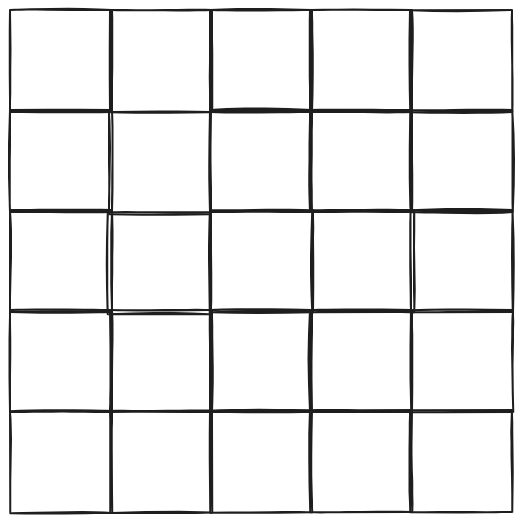
\includegraphics[width=0.5\textwidth]{grade_2d.png}
    \caption{\small Exemplo de autômato celular 2D (5 x 5) com células representando vazios.}
    \label{fig:grade_2d}
\end{figure}

As células interagem com suas vizinhas imediatas, que podem ser definidas de diferentes maneiras. A vizinhança mais comum é a \textit{vizinhança de von Neumann}, que inclui as quatro células adjacentes (cima, baixo, esquerda e direita) pintadas de azul na Figura \ref{fig:vizinhanca_von_neumann}. A \textit{vizinhança de von Neumann estendida}, por sua vez, inclui também as células pintadas de verde na Figura \ref{fig:vizinhanca_von_neumann_estendida}, totalizando oito células vizinhas. Também é possível definir outras vizinhanças, como a \textit{vizinhança de Moore}, que inclui todas as oito células adjacentes (cima, baixo, esquerda, direita e as quatro diagonais), como na Figura \ref{fig:vizinhanca_moore}. A escolha da vizinhança influencia diretamente a dinâmica do autômato celular e, consequentemente, o comportamento emergente do sistema simulado. Neste trabalho são utilizadas as vizinhanças de von Neumann e von Neumann estendida.

\begin{figure}[H]
    \centering
    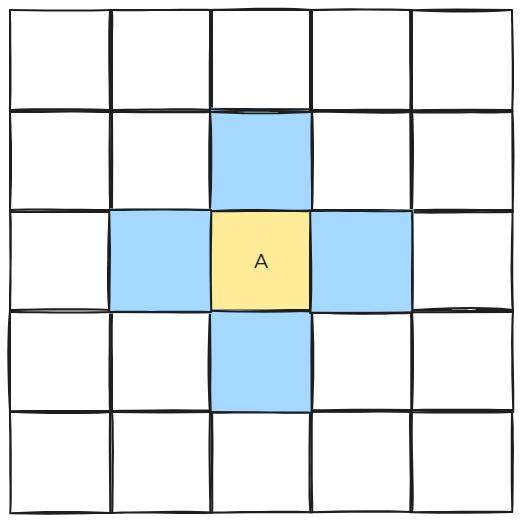
\includegraphics[width=0.5\textwidth]{vizinhanca_von_neumann.png}
    \caption{\small Vizinhança de von Neumann de um componente A, definida pelas 4 células azuis.}
    \label{fig:vizinhanca_von_neumann}
\end{figure}

\begin{figure}[H]
    \centering
    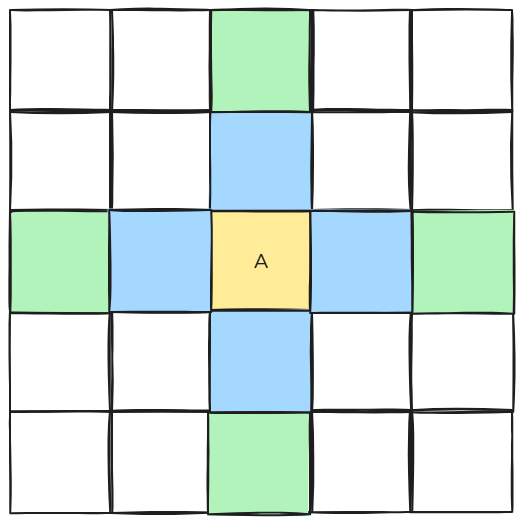
\includegraphics[width=0.5\textwidth]{vizinhanca_von_neumann_estendida.png}
    \caption{\small Vizinhança de von Neumann estendida de um componente A, definida pelas células azuis e verdes.}
    \label{fig:vizinhanca_von_neumann_estendida}
\end{figure}

\begin{figure}[H]
    \centering
    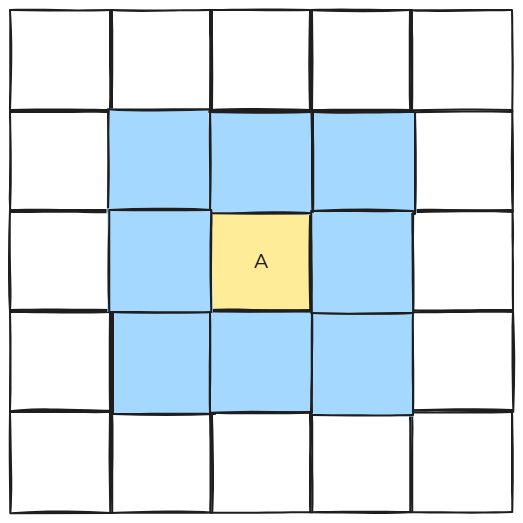
\includegraphics[width=0.5\textwidth]{vizinhanca_moore.png}
    \caption{\small Vizinhança de Moore de um componente A, definida pelas 8 células azuis.}
    \label{fig:vizinhanca_moore}
\end{figure}

Os modelos de autômato celular (AC) empregados neste trabalho seguem predominantemente o formalismo probabilístico descrito por Kier \cite{kier2005}. Cada componente ou vazio ocupa uma célula de uma malha quadrada e interage apenas com as células de sua \textit{vizinhança de von Neumann estendida}. A dinâmica emerge da aplicação sincrônica, a cada iteração, (i) das \textbf{regras de movimentação} e (ii) das \textbf{regras de transição}. A seguir são definidos os quatro parâmetros fundamentais desses conjuntos de regras: $P_m$, $P_b$, $J$ e $P_r$.

\subsubsection{Probabilidade de Movimentação Livre – \texorpdfstring{$P_m$}{Pm}}
\label{sec:probabilidade_movimento_livre}

\begin{itemize}
    \item \textbf{Definição:} $P_m$ representa a chance de um componente isolado se mover para uma célula desocupada de sua vizinhança de von Neumann (Figura \ref{fig:movimentacao_livre}). Essa probabilidade é influenciada por fatores como a densidade de componentes nas células vizinhas e a natureza do próprio componente.
    \item \textbf{Intervalo:} $0 \le P_m \le 1$.
    \item \textbf{Interpretação física:} controla a \textit{mobilidade inerente}.
          Valores próximos de 1 reproduzem um passeio aleatório praticamente livre; valores
          menores simulam espécies mais lentas.
\end{itemize}

\begin{figure}[H]
    \centering
    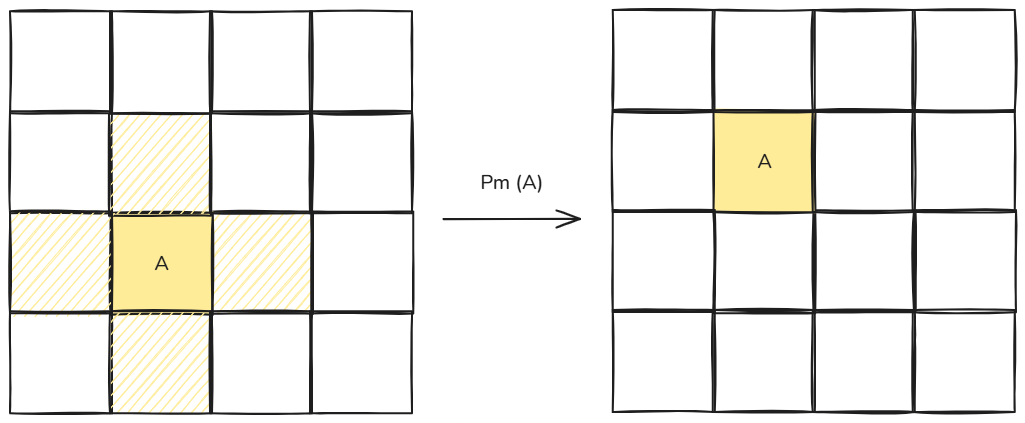
\includegraphics[width=0.8\textwidth]{Pm.png}
    \caption{\small Exemplo de movimentação livre de um componente A para uma célula vazia da sua vizinhança de von Neumann.}
    \label{fig:movimentacao_livre}
\end{figure}

\subsubsection{Parâmetro de Junção – \texorpdfstring{$J$}{J}}
\label{subsubsec:J}

\begin{itemize}
    \item \textbf{Definição:} $J(AB)$ modula a
          \emph{propensão de movimento de $A$ na direção de $B$}
          quando ambos estão separados por exatamente uma célula vazia. A Figura \ref{fig:movimentacao_juncao} ilustra essa situação, onde $A$ possui um vazio em sua vizinhança de von Neumann e este vazio separa $A$ de $B$ que, por sua vez, está na vizinhança de von Neumann estendida de $A$.
    \item \textbf{Valores típicos:}
          \[
              J(AB)=
              \begin{cases}
                  >1    & \text{atração curta distância}  \\[2pt]
                  =1    & \text{deslocamento indiferente} \\[2pt]
                  0<J<1 & \text{repulsão}                 \\[2pt]
                  =0    & \text{movimento proibido}
              \end{cases}
          \]
    \item \textbf{Significado químico:} descreve interações
          hidrofóbicas/hidrofílicas, cargas opostas, etc.
          Por exemplo, \citeauthor{kier2005} ajustam
          $J(\mathrm{WW})>1$ para reproduzir a coesão da água líquida.
\end{itemize}

\begin{figure}[H]
    \centering
    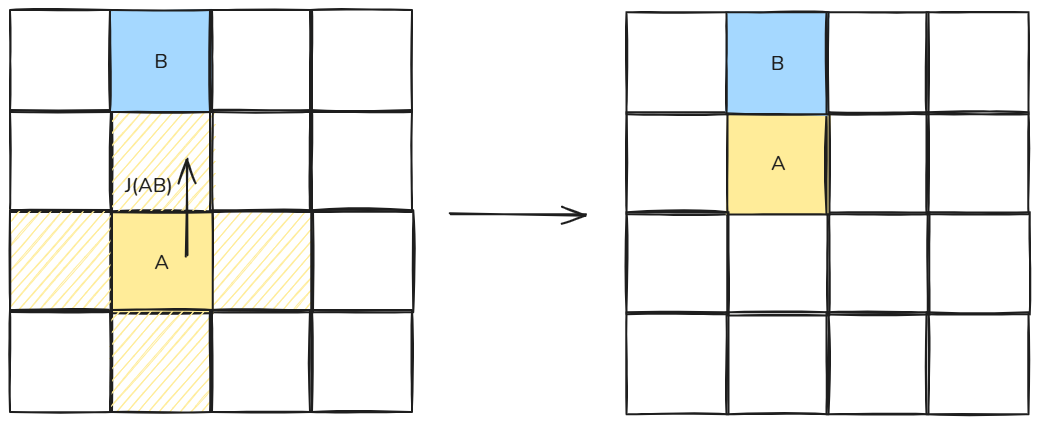
\includegraphics[width=0.8\textwidth]{Jab.png}
    \caption{\small Exemplo de movimentação de um componente A na direção de um componente B, separados por uma célula vazia, com propensão de movimento $J(AB)$.}
    \label{fig:movimentacao_juncao}
\end{figure}

\subsubsection{Probabilidade de Quebra – \texorpdfstring{$P_b$}{Pb}}
\label{subsubsec:Pb}

\begin{itemize}
    \item \textbf{Definição:} $P_b(AB)$ é a probabilidade de
          \emph{separação} de dois componentes adjacentes $A$ e $B$
          (``quebra de ligação'') em uma iteração. A Figura \ref{fig:quebra_ligacao} ilustra essa situação, onde $B$ está em uma célula adjacente a $A$.
    \item \textbf{Intervalo:} $0 \le P_b \le 1$.
    \item \textbf{Coesão:} $P_b=0$ \,($A$ e $B$ nunca se separam)
          $\rightarrow$ forte coesão;
          $P_b=1$ \,($A$ e $B$ sempre se separam) $\rightarrow$ ligação fraca.
    \item \textbf{Dependência de coordenação:} se $A$ está ligado a
          $n$ vizinhos do tipo $B$, a probabilidade conjunta de separação é
          $P_b^{\,n}$; logo, múltiplos contatos estabilizam o agregado.
    \item \textbf{Correspondência físico-química:}
          em água, $P_b(\mathrm{WW})$ pode ser correlacionado com a temperatura:
          valores maiores a temperaturas elevadas representam a maior
          desordem da rede de ligações de hidrogênio \cite{kier2005}.
\end{itemize}

\begin{figure}[H]
    \centering
    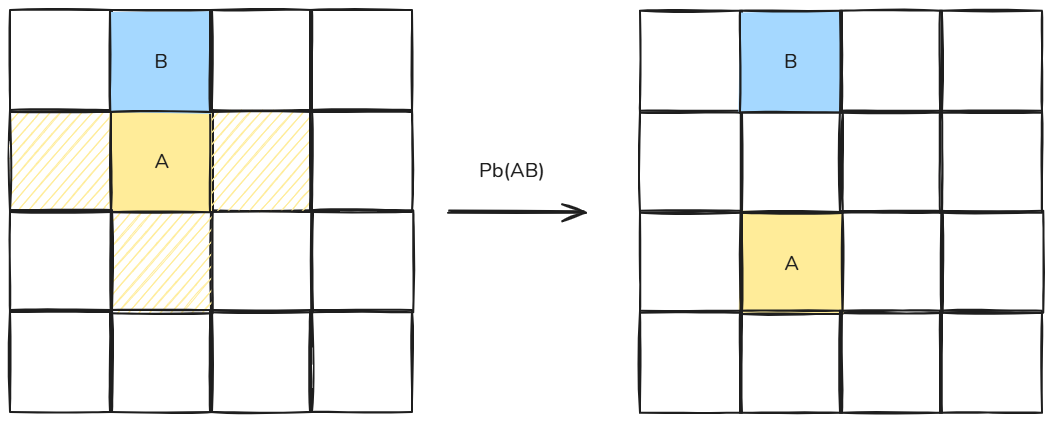
\includegraphics[width=0.8\textwidth]{PbAB.png}
    \caption{\small Exemplo de quebra de ligação entre dois componentes A e B adjacentes, com probabilidade de quebra $P_b(AB)$.}
    \label{fig:quebra_ligacao}
\end{figure}

\subsubsection{Probabilidade de Reação – \texorpdfstring{$P_r$}{Pr}}
\label{subsubsec:Pr}

\begin{itemize}
    \item \textbf{Definição:} $P_r$ (substitui o símbolo $P_t$ de
          \citeauthor{kier2005}) é a probabilidade de conversão química
          durante uma iteração. A Figura \ref{fig:reacao} ilustra essa situação, onde $A$ e $B$ estão em células adjacentes e podem reagir para formar $C$ e $D$.
    \item \textbf{Intervalo:} $0 \le P_r \le 1$.
    \item \textbf{Reações elementares:} $P_r$ é aplicado a
          \emph{reações elementares} que ocorrem quando
          dois componentes estão em células adjacentes.
          Por exemplo, $A+B \xrightarrow{P_r(AB)} C+D$
          representa a reação entre $A$ e $B$ para formar $C$ e $D$ com probabilidade $P_r(AB)$.
    \item \textbf{Casos de uso:}
          \begin{enumerate}
              \item \emph{Transição de primeira ordem:}
                    $A \xrightarrow{P_r(A\rightarrow B)} B$.\\
                    Se $P_r=1$ a transição é determinística;
                    $0<P_r<1$ torna-a estocástica.
              \item \emph{Reação de encontro (segunda ordem):}\\
                    quando $A$ e $B$ tornam-se vizinhos,
                    ocorre $A+B \xrightarrow{P_r(AB)} C+D$
                    com probabilidade $P_r(AB)$.
          \end{enumerate}
    \item \textbf{Significado cinético:} $P_r$ pode ser relacionado a
          uma constante de velocidade efetiva $k$
          (\textit{via} calibração: $k = P_r/\Delta t$,
          onde $\Delta t$ é a duração de uma iteração).
    \item \textbf{Importância prática:}
          em modelos enzimáticos, por exemplo, $P_r(\mathrm{AB})$
          controla a etapa catalítica $\mathrm{ES}\rightarrow\mathrm{EP}$
          e permite reproduzir curvas de Michaelis–Menten
          \cite[cap.~9]{kier2005}.
\end{itemize}

\begin{figure}[H]
    \centering
    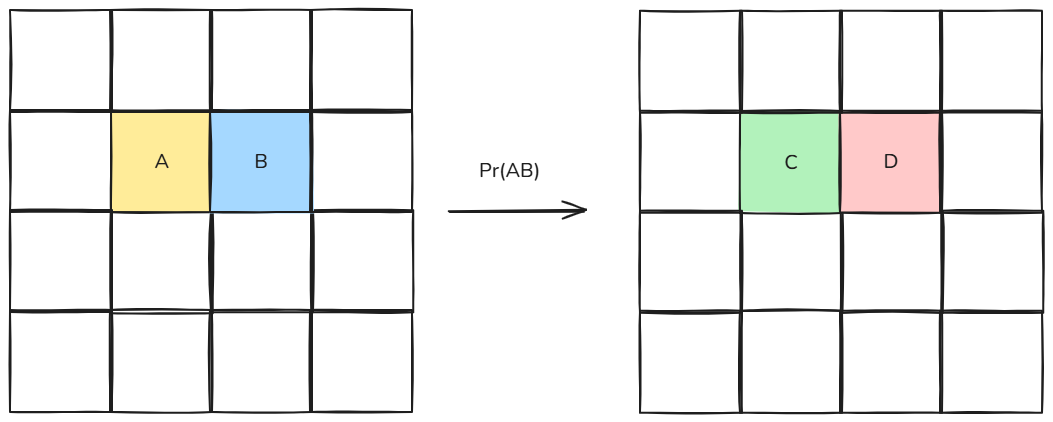
\includegraphics[width=0.8\textwidth]{reacao.png}
    \caption{\small Exemplo de reação entre dois componentes A e B adjacentes, formando C e D com probabilidade de reação $P_r(AB)$.}
    \label{fig:reacao}
\end{figure}

\begin{table}[H]
    \centering
    \caption{\textbf{Parâmetros Fundamentais do Modelo de Autômato Celular}}
    \vspace{0.2cm}
    \begin{tabularx}{\textwidth}{X m{3cm} m{3cm}}
        \hline
        \textbf{Parâmetro}                  & \textbf{Símbolo} & \textbf{Intervalo}  \\
        \hline
        Probabilidade de movimentação livre & $P_m$            & $0 \leq P_m \leq 1$ \\
        Probabilidade de quebra             & $P_b$            & $0 \leq P_b \leq 1$ \\
        Parâmetro de junção                 & $J$              & $0 \leq J < \infty$ \\
        Probabilidade de reação             & $P_r$            & $0 \leq P_r \leq 1$ \\
        \hline
    \end{tabularx}

    \vspace{0.2cm}
    \makebox[\linewidth][l]{\small Fonte: Autoria própria}
\end{table}

\subsection{Simulação de Reações Químicas}

A simulação de reações químicas é um campo crucial para a compreensão e otimização de processos industriais e biológicos. Tradicionalmente, a cinética química é modelada por meio de equações diferenciais ordinárias (EDOs) que descrevem a variação das concentrações dos reagentes e produtos ao longo do tempo. Essas abordagens, baseadas em leis de velocidade e constantes cinéticas, são eficazes para sistemas homogêneos e bem misturados, onde as concentrações podem ser consideradas uniformes em todo o volume reacional. No entanto, em sistemas heterogêneos, onde a difusão e os efeitos espaciais desempenham um papel significativo, as EDOs podem não ser suficientes para capturar a complexidade do sistema. Nesses casos, métodos baseados em simulação estocástica, como o algoritmo de Gillespie, ou abordagens baseadas em elementos finitos, que discretizam o espaço e resolvem equações diferenciais parciais, são frequentemente empregados para considerar a distribuição espacial das espécies químicas \cite{Gillespie1977}.

Os autômatos celulares oferecem uma alternativa promissora para a simulação de reações químicas, especialmente em sistemas onde a localização espacial e a difusão são importantes. Em um modelo de AC para reações químicas, cada célula da grade pode representar um pequeno volume do espaço reacional e conter um conjunto de "partículas" ou "moléculas" que representam as espécies químicas. As regras de transição do autômato celular são então projetadas para simular os processos elementares que ocorrem no sistema: difusão e reação. A difusão é modelada permitindo que as partículas se movam entre células vizinhas, geralmente com uma certa probabilidade. As reações químicas são simuladas quando partículas de diferentes espécies ocupam a mesma célula ou células adjacentes, e as regras de transição definem como essas partículas interagem para formar novos produtos, com probabilidades que refletem as constantes de velocidade das reações \cite{kier2005}.

A grande vantagem dos autômatos celulares na simulação de reações químicas reside na sua capacidade de incorporar explicitamente a heterogeneidade espacial e os efeitos de difusão de forma natural. Ao contrário das abordagens baseadas em EDOs, que assumem homogeneidade, os ACs permitem que as concentrações das espécies variem localmente, e que as reações ocorram apenas onde os reagentes estão presentes. Isso é particularmente útil para sistemas onde a mistura não é perfeita, ou onde existem gradientes de concentração significativos, como em reações em superfícies, em géis ou em sistemas biológicos. Além disso, os ACs podem simular a estocasticidade inerente às reações químicas em nível molecular, onde as interações são probabilísticas. A natureza discreta e paralela dos autômatos celulares também os torna adequados para implementação em computadores, permitindo a simulação de sistemas complexos com um grande número de partículas e células \cite{kier2005}.

Um exemplo clássico da aplicação de autômatos celulares em reações químicas é a simulação de reações de Belousov-Zhabotinsky, que exibem padrões oscilatórios e ondas de propagação. Nesses modelos, as regras de transição são formuladas para replicar as interações químicas que levam a esses comportamentos complexos, e os ACs conseguem reproduzir fielmente os padrões observados experimentalmente. Outras aplicações incluem a simulação de reações em catálise heterogênea, onde a superfície do catalisador pode ser representada por uma grade de células, e as moléculas reagentes se adsorvem, reagem e dessorvem de acordo com as regras do autômato. A flexibilidade dos autômatos celulares permite a incorporação de diversos fatores, como a temperatura, a presença de inibidores ou ativadores, e a geometria do reator, tornando-os uma ferramenta versátil para a exploração de fenômenos cinéticos complexos \cite{kier2005}.

\subsection{Simulação de Reações Enzimáticas com Autômatos Celulares}

\subsubsection{Trabalho de Vasconcelos}

O objetivo central do trabalho de Vasconcelos \cite{vasconcelos2019} foi construir um modelo de autômatos celulares (AC) capaz de reproduzir a cinética enzimática de Michaelis–Menten e variações mais complexas sem recorrer a equações diferenciais. Para isso, o autor partiu de uma malha quadrada 2-D de 100 × 100 sítios com contorno toroidal, de modo que cada célula pode conter exatamente um componente químico ($E$, $S$, $P$, complexos ou “água”) e interagir apenas com seus quatro vizinhos de von Neumann.

A primeira etapa metodológica buscou validar uma nova forma de representar o complexo enzima-substrato. Em vez de um estado único, o autor utilizou duas células adjacentes ligadas por restrições de quebra quase nulas. O objetivo era manter a integridade espacial do complexo durante as iterações e, ao mesmo tempo, facilitar sua dissociação controlada. Quando comparada a um modelo clássico de um único passo ($E + S \rightarrow E + P$), a abordagem bivizinha produziu curvas de formação de produto praticamente sobrepostas, com diferença inferior a 1 $\%$ em toda a simulação, confirmando a equivalência cinética das duas representações.

Com essa validação em mãos, a pesquisa avançou para analisar o efeito da concentração inicial de substrato. Ao variar gradualmente a quantidade de $S$, Vasconcelos observou um aumento nítido no pico de enzima complexada e um prolongamento da fase pré-estacionária. Em números, o máximo de $ES$ praticamente dobrou entre a menor e a maior carga de substrato, enquanto o tempo para que a enzima retornasse majoritariamente ao estado livre cresceu de poucas centenas para cerca de duas mil iterações. Esses comportamentos reproduzem qualitativamente a dependência entre saturação enzimática e disponibilidade de substrato descrita pelos modelos contínuos.

Para verificar se as simulações poderiam fornecer parâmetros globais, foi aplicado o método de Lineweaver–Burk aos valores de velocidade inicial extraídos de oito grupos de ensaios. A regressão linear exibiu coeficiente de determinação $R^2 \approx 0,97$, indicando forte aderência à equação de Michaelis–Menten. A interseção das retas revelou $V_{max}$ em torno de 0,026 fração de produto por iteração (equivalente a cerca de 260 moléculas por passo) e um $K_M$ próximo de 9 unidades relativas de substrato, números compatíveis com sistemas reais quando se normaliza a escala discreta do autômato.

Em seguida, o algoritmo foi estendido para testar diferentes mecanismos de inibição. A inclusão de um inibidor competitivo, modelado como nova espécie com afinidade exclusiva pela enzima livre, reduziu a conversão final de produto para cerca de 29 \%. No cenário de inibição irreversível, onde o complexo $EI$ não se desfazia mais, o rendimento caiu ainda mais, estabilizando próximo de 18 \%. Por contraste, a reação de Michaelis–Menten sem inibidor atingiu perto de 52 \% de conversão, enquanto a variante reversível ($E + P \rightleftharpoons ES$) apresentou um perfil mais lento, mas alcançou 45 \% ao final da janela analisada, evidenciando a recombinação do produto à enzima.

Os traços temporais dessas quatro configurações mostraram assinaturas distintas: nas curvas competitivas, a desaceleração ocorreu logo no início, refletindo a competição direta por sítios ativos; na rota irreversível, a atividade declinou continuamente à medida que a fração de enzima funcional era sequestrada em $EI$; e na versão reversível, observou-se uma queda inicial seguida de leve recuperação, resultado da reciclagem do produto.

Para avaliar a flexibilidade do modelo, o capítulo final abordou a cinética ping-pong bi-bi típica de lipases. Foram introduzidas duas formas enzimáticas ($E_1 e E_2$) e seus respectivos complexos com substratos diferentes. Mesmo com essa rede de etapas adicionais, o autômato manteve estabilidade numérica e converteu mais de 90 \% dos substratos em menos de mil iterações. O consumo sequencial — primeiro $S_1$, depois $S_2$ — surgiu espontaneamente, replicando a alternância de estados catalíticos característica do mecanismo.

O conjunto de resultados confirma que regras locais simples podem gerar a dinâmica global descrita pela teoria enzimática clássica, inclusive parâmetros cinéticos mensuráveis. Além disso, o modelo dispensou a hipótese de estado estacionário, pois acompanhou explicitamente as flutuações de $E$, $ES$ e outros intermediários ao longo de todo o processo.

Outro aspecto relevante foi o uso exclusivo de software livre (\textit{NumPy}, \textit{Pandas}, \textit{Matplotlib}), demonstrando que a abordagem possui baixo custo de implementação e é acessível para pesquisas acadêmicas ou ensino de Engenharia Química e Bioquímica.

Em última análise, o trabalho de Vasconcelos mostra que autômatos celulares constituem uma alternativa robusta para estudar cinética enzimática, permitindo não só reproduzir quantitativamente curvas familiares, mas também explorar cenários onde dados experimentais são escassos ou onde o tratamento diferencial se torna impalpável.

\subsubsection{Trabalho de Dutta}

O artigo de Dutta et al. \cite{dutta2015generalized} apresenta uma abordagem original ao utilizar autômatos celulares (AC) para simular a cinética enzimática de primeira ordem, superando algumas limitações dos modelos baseados em equações diferenciais ordinárias. Ao concentrar-se em representações discretas e estocásticas, o estudo justifica a importância de considerar a heterogeneidade espacial e as flutuações inerentes aos sistemas bioquímicos, especialmente em escalas micro e mesoscópicas.

A metodologia adotada pelos autores baseia-se na construção de uma grade bidimensional, na qual cada célula representa uma porção do sistema reacional contendo enzimas, substratos e produtos. Nesta configuração, os estados das células são discretos, e a evolução temporal do sistema é determinada por regras de transição probabilísticas que simulam as reações enzimáticas. A aplicação de tais regras locais, que levam em conta a vizinhança de von Neumann estendida, permite que o modelo capte não apenas os aspectos cinéticos, mas também os efeitos difusivos e a propagação de informações entre células adjacentes.

Um dos pontos centrais do trabalho reside na incorporação da estocasticidade, característica intrínseca dos sistemas biológicos com número reduzido de moléculas. Diferente dos modelos determinísticos, essa abordagem permite a observação de flutuações e padrões emergentes que se manifestam quando o sistema opera em regimes de baixa concentração, oferecendo uma representação mais realista dos fenômenos enzimáticos. Além disso, a flexibilidade do modelo possibilita a adaptação dos parâmetros para simular diferentes cenários de inibição enzimática, como os mecanismos competitivos e alostéricos.

Para demonstrar a eficácia do método proposto, os autores realizaram um conjunto de simulações que compararam os resultados obtidos com as soluções clássicas das equações diferenciais. As simulações evidenciaram que, em condições onde o número de moléculas é suficientemente alto, os resultados do modelo de autômatos celulares convergem para os preditos pelos métodos determinísticos. Entretanto, em sistemas de menor dimensão, as discrepâncias tornam-se evidentes, ressaltando a importância dos efeitos estocásticos e a vantagem da abordagem AC para a compreensão de sistemas com alta sensibilidade a variações locais.

Outra contribuição relevante do estudo é a realização de uma análise de sensibilidade dos parâmetros do modelo. Ao variar as probabilidades de reação e o tamanho da grade, os autores verificaram que o comportamento do sistema pode ser significativamente alterado, especialmente em regimes onde a difusão e a interação local são determinantes para a dinâmica global. Essa análise reforça a robustez do modelo, ao mesmo tempo em que aponta para a necessidade de uma calibração cuidadosa dos parâmetros quando se pretende aplicar o método a sistemas experimentais ou industriais.

Em síntese, o trabalho de Dutta et al. \cite{dutta2015generalized} evidencia que autômatos celulares podem oferecer uma ferramenta poderosa e flexível para a simulação de cinéticas enzimáticas de primeira ordem, permitindo a captura de nuances que os modelos tradicionais não contemplam. A abordagem proposta amplia as possibilidades de modelagem em bioengenharia, possibilitando estudos mais refinados sobre a natureza dos processos enzimáticos e sugerindo novas direções para pesquisas futuras na área. Essa perspectiva pode ser especialmente útil em aplicações que envolvem microreatores, bioprocessos e a investigação de mecanismos de inibição enzimática.

\subsubsection{Trabalho de Weimar}

O artigo de Weimar \cite{weimar2002cellular} apresenta uma abordagem inovadora para a simulação de redes de reações enzimáticas por meio de autômatos celulares, desafiando os métodos tradicionais baseados em equações diferenciais ordinárias. O autor parte da premissa de que a modelagem determinística pode não capturar com fidelidade os efeitos espaciais e estocásticos, comuns em sistemas bioquímicos complexos. A proposta de utilizar autômatos celulares permite a discretização do espaço e a implementação de regras locais que simulam, de forma determinística ou probabilística, os eventos de reações químicas em escalas microscópicas.

Na metodologia apresentada, o espaço de simulação é dividido em uma grade bidimensional onde cada célula representa uma região capaz de abrigar diferentes espécies químicas – como substratos, produtos e enzimas. As reações enzimáticas são modeladas através de regras de transição que incorporam as taxas das reações, inspiradas nos modelos clássicos, como o de Michaelis-Menten. Essa abordagem permite que o sistema possa evoluir em etapas discretas de tempo, onde cada iteração reflete a possibilidade de ocorrência ou não de uma reação, considerando a proximidade dos reagentes e as condições locais.

Weimar propõe uma representação estocástica para os processos enzimáticos, o que possibilita a captura de flutuações locais de concentração e a emergência de padrões espaciais não previstos por modelos contínuos. Nesse cenário, as regras de transição do autômato são definidas com base em probabilidades, que refletem as constantes cinéticas experimentais. Essa modelagem probabilística ressalta a relevância do acaso e da heterogeneidade na dinâmica dos sistemas enzimáticos, proporcionando uma visão mais realista do comportamento dos sistemas quando comparados aos modelos baseados em equações diferenciais.

Os resultados apresentados no artigo evidenciam que o uso de autômatos celulares reproduz de maneira consistente o comportamento global esperado das reações enzimáticas, ao mesmo tempo em que revela dinâmicas locais complexas. Entre as descobertas, destacam-se a formação de gradientes de concentração e a ocorrência de eventos de reação que, em conjunto, contribuem para a emergência de padrões espaciais. Essas simulações demonstram que, enquanto os modelos tradicionais focam na média global dos sistemas, o autômato celular consegue detalhar as irregularidades espaciais inerentes aos processos biológicos, indicando uma maior robustez na modelagem de situações heterogêneas.

O autor também discute a capacidade de adaptação do método para simular sistemas mais complexos, como os que envolvem múltiplas enzimas e vias metabólicas interligadas. A flexibilidade do modelo é ressaltada na possibilidade de incorporar diferentes tipos de reações, inibições e cooperações entre as enzimas, alargando seu potencial de aplicação em diversas áreas da bioquímica e engenharia biológica. Assim, a metodologia proposta por Weimar não só contribui para uma melhor compreensão dos mecanismos enzimáticos, mas também abre caminho para a exploração de novos parâmetros e cenários de simulação.

Por fim, embora o artigo aponte algumas limitações relacionadas ao aumento na demanda computacional quando se simula sistemas de grande escala e à complexidade na adequada parametrização das regras do autômato, os benefícios advindos do realismo espacial e da possibilidade de capturar comportamentos emergentes são ressaltados. Conclui-se que o trabalho de Weimar \cite{weimar2002cellular} representa uma contribuição significativa para a área de modelagem de cinética enzimática, destacando os autômatos celulares como uma ferramenta promissora para explorar a dinâmica complexa dos sistemas bioquímicos, especialmente em contextos onde a heterogeneidade espacial é determinante.

\subsubsection{Trabalho de Seybold, Kier e Cheng}

O trabalho de Seybold, Kier e Cheng \cite{seybold1997simulation} representa um avanço significativo no estudo da simulação de reações químicas, especificamente no âmbito das cinéticas de primeira ordem. Os autores propuseram o uso de autômatos celulares como uma ferramenta computacional alternativa aos métodos tradicionais baseados em equações diferenciais. Essa abordagem permite a modelagem detalhada do comportamento de espécies químicas em sistemas discretos, capturando simultaneamente os aspectos determinísticos e as flutuações estocásticas inerentes a reações de escala microscópica.

Na metodologia apresentada, o sistema é representado por uma grade bidimensional onde cada célula simboliza uma unidade reacional. Cada célula pode se encontrar em um dos dois estados possíveis: estado 0, representando o reagente, ou estado 1, correspondendo ao produto formado após a reação. As condições iniciais da simulação são definidas pela distribuição de estados na grade, o que possibilita a análise de diversos cenários e a avaliação da evolução temporal da reação mediante diferentes configurações.

O mecanismo central do modelo é a transição estocástica das células, regida por uma probabilidade de conversão do reagente (estado 0) para o produto (estado 1). Essa probabilidade, $P$, é calculada a partir da constante de velocidade da reação, $k$, e do intervalo de tempo, $\Delta t$, segundo a fórmula

\begin{equation}
    P = 1 - e^{-k \Delta t}
\end{equation}

O caráter estocástico é reforçado pela implementação de atualizações assíncronas, onde cada célula é avaliada de maneira independente em cada etapa do tempo, permitindo que o modelo simule variabilidades que seriam negligenciadas por abordagens puramente determinísticas.

Os resultados demonstrados evidenciam que, para grades com um número expressivo de células, o comportamento médio do sistema converge para as soluções obtidas por métodos determinísticos tradicionais. Em sistemas de menor escala ou em estágios iniciais da reação, entretanto, as flutuações estocásticas são mais pronunciadas, refletindo as variações intrínsecas ao processo reacional. Essa capacidade de transitar entre comportamentos determinísticos e estocásticos ressalta a versatilidade do método e sua adequação para o estudo de processos que apresentam dinâmicas complexas, como as reações enzimáticas.

Outro ponto relevante do estudo é a flexibilidade do modelo, o qual foi aplicado a diversas configurações de reações de primeira ordem, tais como decaimento simples, reações opostas, consecutivas e paralelas. Essa versatilidade não só demonstra o potencial dos autômatos celulares para abranger uma ampla gama de sistemas reacionais, mas também torna a metodologia aplicável em contextos educacionais e experimentais onde a simplicidade computacional é uma demanda. O método proposto, portanto, estabelece uma ponte entre a modelagem teórica e as simulações práticas, contribuindo para a compreensão dos mecanismos subjacentes às reações químicas.

Em síntese, o estudo de Seybold, Kier e Cheng \cite{seybold1997simulation} apresenta uma abordagem inovadora para a simulação de cinéticas químicas utilizando autômatos celulares. Ao integrar a modelagem discreta com regras probabilísticas e atualizações assíncronas, os autores evidenciam uma estratégia eficaz para reproduzir tanto os comportamentos determinísticos quanto as variações estocásticas observadas em reações de primeira ordem. Essa contribuição se destaca pela simplicidade de implementação e pelo potencial de aplicação em estudos mais complexos, estabelecendo as bases para a utilização de autômatos celulares em investigações futuras envolvendo reações enzimáticas e outros processos dinâmicos.

\chapter{METODOLOGIA}

\section{Modelo do Autômato Celular}

\subsection{Definição}

O modelo de AC utilizado neste trabalho é baseado em uma grade 2D, composta por células que podem conter componentes químicos ou vazios. Cada célula pode interagir com suas vizinhas imediatas, definidas pela vizinhança de von Neumann estendida. As regras de movimentação e reação são aplicadas de forma síncrona a todas as células, permitindo que o sistema evolua ao longo do tempo. As regras de evolução são definidas pelos parâmetros $P_m$, $P_b$, $J$ e $P_r$.

A grade é inicializada com uma distribuição aleatória de componentes e vazios. Durante cada iteração, as células são atualizadas conforme as regras do modelo, que consideram os estados das células vizinhas e os parâmetros definidos. O percurso da grade segue uma ordem sistemática: começa na célula superior esquerda (0, 0), avança horizontalmente até a última célula da linha, e então prossegue para a primeira célula da próxima linha (1, 0). Esse padrão se repete até que todas as células da grade sejam processadas. Após a atualização completa da grade, uma iteração do autômato celular é concluída, e o processo reinicia, percorrendo novamente todas as células. Esse ciclo continua até atingir o número de iterações especificado. A Figura \ref{fig:percorre_grade} ilustra o percurso de uma grade 2D 4 x 4 durante uma iteração do autômato celular. Nesse exemplo, a grade é percorrida da célula (0, 0) até a célula (0, 3), pulando para a próxima linha na célula (1, 0) e assim por diante, seguindo a ordem de leitura de uma matriz bidimensional.

\begin{figure}[H]
    \centering
    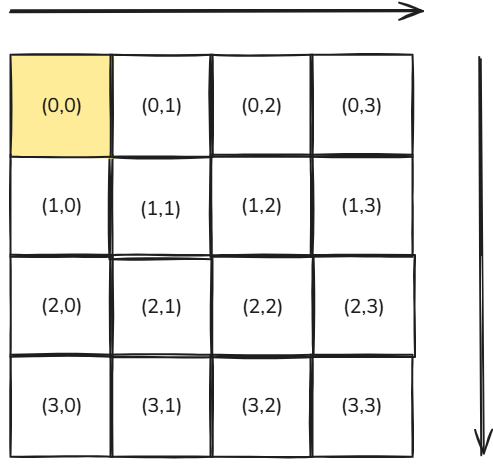
\includegraphics[width=0.5\textwidth]{percorre_grade.png}
    \caption{\small Percurso da grade 2D durante as iterações do autômato celular.}
    \label{fig:percorre_grade}
\end{figure}

A respeito da interação entre as células das bordas da malha, o modelo adota a condição de contorno \textbf{toroidal}, onde as células da borda interagem com as células opostas. Por exemplo, a célula (0, 0) está conectada à célula (0, 3) e, também, à celula (3, 0), fazendo parte de sua vizinhança de von Neumann. Essa abordagem garante que todas as células tenham vizinhos válidos, independentemente de sua posição na malha. Outras condições de contorno, como a cilíndrica e a caixa, também são utilizadas em autômatos celulares, embora neste trabalho a toroidal prevaleça a fim de garantir continuidade e evitar problemas de borda. A condição de contorno cilíndrica conecta as células da borda horizontalmente ou verticalmente, enquanto a caixa trata as bordas como paredes fixas, o que pode limitar a dinâmica do sistema. A Figura \ref{fig:torus} ilustra a condição de contorno toroidal aplicada ao modelo. Nota-se que a vizinhança de von Neumann da célula (0, 0) é composta pelas células (0, 1), (1, 0), (3, 0) e (0, 3).

\begin{figure}[H]
    \centering
    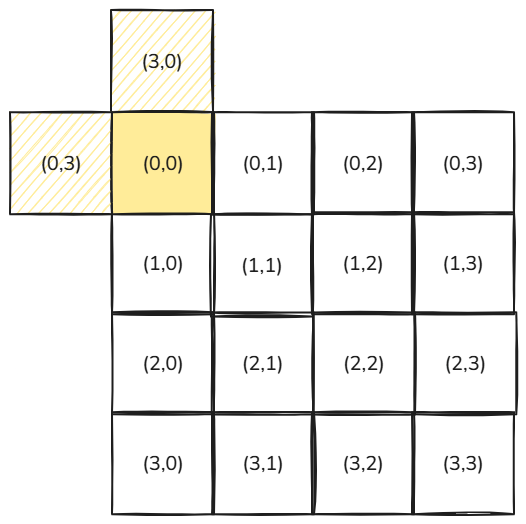
\includegraphics[width=0.5\textwidth]{torus.png}
    \caption{\small Condição de contorno toroidal aplicada ao modelo de autômato celular.}
    \label{fig:torus}
\end{figure}

\subsection{Regras de Evolução}

\section{Implementação Computacional}

\subsection{Código Fonte do Modelo}
% mencionar que você escreveu um código em Python para a simulação (que estará no Apêndice ou no GitHub).
% fluxograma

\subsection{Interface do Usuário}
% explicar como você construiu a interface para o usuário (prints de tela são bem-vindos), inclusive com os detalhes de input/output.

% \begin{figure}[H]
%     \centering
%     \includegraphics[width=0.8\textwidth]{interface_usuario.png}
%     \caption{Interface do Usuário}
%     \label{fig:interface_usuario}
% \end{figure}

\subsection{Ambiente Computacional}
% computador utilizado para as simulações (mencionar especialmente processador e RAM).
% Performance do código (tempo de execução, uso de memória, etc.).


\begin{table}[H]
    \centering
    \caption{\textbf{Interpretação da probabilidade ($P_B$)}}
    \vspace{0.2cm}
    \begin{tabularx}{\textwidth}{m{3.5cm} X}
        \hline
        \multicolumn{2}{c}{$\mathbf{0 \leq P_B(\mathbf{x}_i, \mathbf{x}_j) \leq 1}$} \\
        \hline
        \textbf{Valores} & \textbf{Significado}                                      \\
        \hline
        $P_B = 0$        & Os componentes permanecem sempre unidos                   \\
        $P_B \to 0^+$    & Tendência de permanecerem sempre unidos                   \\
        $P_B \to 1^-$    & Tendência de permanecerem sempre separados                \\
        $P_B = 1$        & Os componentes permanecem sempre separados                \\
        \hline
    \end{tabularx}

    \vspace{0.2cm}
    \makebox[\linewidth][l]{\small Fonte: Autoria própria}
\end{table}

\chapter{RESULTADOS}
% Conteúdo dos resultados...

\chapter{CONCLUSÕES}
% Conclusões finais...

\printbibliography[title={REFERÊNCIAS},heading=bibnumbered]

\appendix

\chapter{Título do Apêndice}
Conteúdo do apêndice...

\chapter{Título do Anexo}
Conteúdo do anexo...

\end{document}

